\documentclass[10pt,landscape,a4paper]{article}
\usepackage[landscape,margin=0.5in]{geometry}
\usepackage{multicol}
\usepackage{amsmath,amssymb}
\usepackage{graphicx}
\usepackage{xcolor}
\usepackage{tikz}
\usepackage{booktabs}
\usepackage{enumitem}
\usepackage{fancyhdr}
\usepackage{titlesec}

% Compact formatting
\setlength{\parindent}{0pt}
\setlength{\parskip}{2pt}
\setlist[itemize]{leftmargin=*, noitemsep, topsep=0pt}
\setlist[enumerate]{leftmargin=*, noitemsep, topsep=0pt}

% Section formatting
\titleformat{\section}{\normalfont\large\bfseries\color{blue!70!black}}{\thesection}{1em}{}
\titleformat{\subsection}{\normalfont\normalsize\bfseries\color{blue!50!black}}{\thesubsection}{1em}{}
\titlespacing*{\section}{0pt}{6pt}{3pt}
\titlespacing*{\subsection}{0pt}{4pt}{2pt}

% Box for important formulas
\newcommand{\importantbox}[1]{%
  \fcolorbox{blue!50!black}{blue!5}{%
    \parbox{0.92\linewidth}{#1}%
  }%
}

% Highlight color
\newcommand{\highlight}[1]{\colorbox{yellow!30}{$#1$}}

\pagestyle{fancy}
\fancyhf{}
\fancyhead[C]{\textbf{Control Theory of Linear Unbranched Chains -- Cheat Sheet}}
\fancyfoot[C]{\thepage}
\renewcommand{\headrulewidth}{0.4pt}

\begin{document}

\begin{multicols}{3}

% =============================================================================
\section{System Structure}
% =============================================================================

\subsection{Unbranched Reaction Chain}

\begin{center}
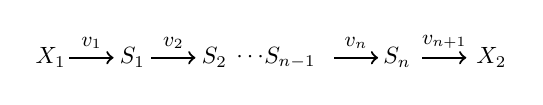
\begin{tikzpicture}[scale=0.8, every node/.style={scale=0.85}]
\node at (0,0) {$X_1$};
\draw[->, thick] (0.3,0) -- (1.0,0) node[midway, above] {\small $v_1$};
\node at (1.3,0) {$S_1$};
\draw[->, thick] (1.6,0) -- (2.3,0) node[midway, above] {\small $v_2$};
\node at (2.6,0) {$S_2$};
\node at (3.2,0) {$\cdots$};
\node at (3.8,0) {$S_{n-1}$};
\draw[->, thick] (4.5,0) -- (5.2,0) node[midway, above] {\small $v_n$};
\node at (5.5,0) {$S_n$};
\draw[->, thick] (5.9,0) -- (6.6,0) node[midway, above] {\small $v_{n+1}$};
\node at (7.0,0) {$X_2$};
\end{tikzpicture}
\end{center}

\begin{itemize}
\item $X_1$ = external substrate (constant)
\item $X_2$ = external product (constant)
\item $S_1, \ldots, S_n$ = internal metabolites
\item $v_1, \ldots, v_{n+1}$ = reaction rates
\item $r = n+1$ = number of reactions
\end{itemize}

\subsection{Steady-State Property}

\importantbox{
At steady state, all reaction rates equal the flux:
\begin{equation*}
v_j = J \quad \text{for } j = 1, \ldots, n+1
\end{equation*}
}

\textbf{Key consequence:} The flux control coefficient matrix has identical rows:
\[
C_j^J = C_{ij}^J \quad \text{for all } i
\]

% =============================================================================
\section{Linear Kinetics (Non-Saturated)}
% =============================================================================

\subsection{Conditions for Linear Regime}

When enzymes operate far from saturation:
\begin{align*}
J &\ll V_j^f, V_j^r \\
S_i &\ll K_i^r, K_{i+1}^f
\end{align*}

$V_j^f$is the forward maximal rate and $V_j^r$ the reverse maximal rate.

$K_i^r$ is the product $K_m$ for the producing step $i$, and $K_{i+1}^f$ is the $K_m$ for the substrate of the consuming step.

Under these conditions we can approximate rate laws using a linear rate law.
\subsection{Linear Rate Law}

\importantbox{
\begin{equation*}
v_j = k_j S_{j-1} - k_{-j} S_j = k_j\left(S_{j-1} - \frac{S_j}{q_j}\right)
\end{equation*}
}

where:
\begin{align*}
k_j &= \frac{V_j^f}{K_j^f} \quad \text{(forward rate constant)} \\[4pt]
k_{-j} &= \frac{V_j^r}{K_j^r} \quad \text{(backward rate constant)} \\[4pt]
q_j &= \frac{k_j}{k_{-j}} = \frac{V_j^f K_j^r}{V_j^r K_j^f} \quad \text{(equilibrium constant)}
\end{align*}

The last relation is the \textbf{Haldane relationship}.

\subsection{Metabolite Concentrations}

\begin{equation*}
S_i = P_1 \prod_{j=1}^{i} q_j - J \sum_{l=1}^{i} \frac{1}{k_l} \prod_{j=l}^{i} q_j
\end{equation*}

\subsection{Steady-State Flux}

\importantbox{
\begin{equation*}
J = \frac{X_1 \displaystyle\prod_{j=1}^{n+1} q_j - X_2}{\displaystyle\sum_{l=1}^{n+1} \frac{1}{k_l} \prod_{j=l}^{n+1} q_j}
\end{equation*}
}

\vspace{2pt}
\textbf{Interpretation:}
\begin{itemize}
\item Numerator: thermodynamic driving force
\item Denominator: sum of resistances weighted by downstream equilibria
\end{itemize}

% =============================================================================
\section{Flux Control Coefficients}
% =============================================================================

\subsection{Definition via Rate Constants}

\begin{equation*}
C_j^J = \frac{k_j}{J} \frac{\partial J}{\partial k_j} = \frac{v_j}{J} \frac{\partial J / \partial k_j}{\partial v_j / \partial k_j}
\end{equation*}

(Perturbation keeps equilibrium constants fixed)

\subsection{Explicit Formula (Linear Kinetics)}

\importantbox{
\begin{equation*}
C_i^J = \frac{\displaystyle\frac{1}{k_i} \prod_{j=i}^{n+1} q_j}{\displaystyle\sum_{l=1}^{n+1} \frac{1}{k_l} \prod_{j=l}^{n+1} q_j}
\end{equation*}
}

\subsection{Fundamental Properties}

\begin{align*}
0 \leq C_j^J &\leq 1 \quad \text{(non-negative, bounded)}\\[4pt]
\sum_{j=1}^{n+1} C_j^J &= 1 \quad \text{(summation theorem)}
\end{align*}

\textbf{Note:} Normalization doesn't change values since $v_j = J$ at steady state.

\vspace{4pt}
\subsection{Ratio of Control Coefficients}

\importantbox{
\begin{equation*}
\frac{C_j^J}{C_i^J} = \frac{k_i}{k_j} \prod_{l=j}^{i-1} q_l \quad \text{with } i > j
\end{equation*}
}

\vspace{4pt}
\textbf{Key insight:} If reaction $s$ is irreversible ($q_s \to \infty$), then $C_i^J \to 0$ for all reactions $i > s$ downstream.

\subsection{Interpretation}

\begin{itemize}
\item Fast reactions ($k_j$ large) $\Rightarrow$ low $C_j^J$
\item Slow reactions ($k_j$ small) $\Rightarrow$ high $C_j^J$
\item Position in chain matters via $\prod q_j$ terms
\item Irreversible steps ``shield'' downstream reactions
\end{itemize}

%\columnbreak

% =============================================================================
\section{Finite Perturbations}
% =============================================================================

\subsection{Single Reaction Perturbation}

\importantbox{
\begin{equation*}
\frac{\Delta J}{J} = \frac{C_k^J \,\Delta v_k / v_k}{1 + (1 - C_k^J)\, \Delta v_k / v_k}
\end{equation*}
}

This exact result applies to unbranched chains with linear kinetics.

\subsection{Multiple Perturbations}

\begin{equation*}
\frac{\Delta J}{J} = \sum_{j=1}^{n+1} C_j^J \left(\frac{\Delta v_j / v_j}{1 + \Delta v_j / v_j}\right) \left(\sum_{j=1}^{n+1} \frac{C_j^J}{1 + \Delta v_j / v_j}\right)^{-1}
\end{equation*}

\subsection{Linear Approximation}

For small perturbations ($|\Delta v_j / v_j| \ll 1$):
\begin{equation*}
\frac{\Delta J}{J} \approx \sum_{j=1}^{n+1} C_j^J \frac{\Delta v_j}{v_j}
\end{equation*}

% =============================================================================
\section{General Treatment (Nonlinear)}
% =============================================================================

\subsection{Elasticity Structure}

For unbranched chains where $v_i$ depends only on $S_{i-1}$ (substrate) and $S_i$ (product):

\begin{equation*}
\varepsilon_{ij} = \varepsilon_{ii}\, \delta_{ij} + \varepsilon_{i,i-1}\, \delta_{i-1,j}
\end{equation*}

\textbf{Typical signs:}
\begin{align*}
\varepsilon_{ii} &< 0 \quad \text{(product inhibition)} \\
\varepsilon_{i+1,i} &> 0 \quad \text{(substrate activation)}
\end{align*}

\subsection{Two-Enzyme System}

\begin{center}
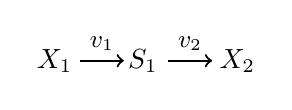
\begin{tikzpicture}[scale=0.8]
\node at (0,0) {$X_1$};
\draw[->, thick] (0.4,0) -- (1.1,0) node[midway, above] {\small $v_1$};
\node at (1.4,0) {$S_1$};
\draw[->, thick] (1.8,0) -- (2.5,0) node[midway, above] {\small $v_2$};
\node at (2.9,0) {$X_2$};
\end{tikzpicture}
\end{center}

\textbf{Flux control:}

\fcolorbox{blue!50!black}{blue!5}{\parbox{0.88\linewidth}{%
\vspace{-8pt}
\begin{align*}
C_1^J &= \frac{\varepsilon_{21}}{\varepsilon_{21} - \varepsilon_{11}} \\[2pt]
C_2^J &= \frac{-\varepsilon_{11}}{\varepsilon_{21} - \varepsilon_{11}}
\end{align*}
\vspace{-12pt}
}}

\textbf{Concentration control:}
\begin{align*}
C_{11}^S &= \frac{1}{\varepsilon_{21} - \varepsilon_{11}} \\[4pt]
C_{12}^S &= \frac{-1}{\varepsilon_{21} - \varepsilon_{11}}
\end{align*}

\subsection{Connectivity Theorem (Unbranched)}

\importantbox{
\begin{equation*}
C_i^J \varepsilon_{ii} + C_{i+1}^J \varepsilon_{i+1,i} = 0
\end{equation*}
}

\vspace{2pt}
\textbf{Rearranged:}
\begin{equation*}
\frac{C_i^J}{C_{i+1}^J} = -\frac{\varepsilon_{i+1,i}}{\varepsilon_{ii}}
\end{equation*}

\subsection{General Flux Control Formula}

\importantbox{
\begin{equation*}
C_i^J = \frac{\displaystyle\prod_{j=i}^{n}\left(-\frac{\varepsilon_{j+1,j}}{\varepsilon_{jj}}\right)}{1 + \displaystyle\sum_{j=1}^{n} \prod_{l=j}^{n}\left(-\frac{\varepsilon_{l+1,l}}{\varepsilon_{ll}}\right)}
\end{equation*}
}

\vspace{4pt}
When $\varepsilon_{ii} < 0$ and $\varepsilon_{i+1,i} > 0$, all $C_j^J \geq 0$.

\subsection{Implications for Enzyme Properties}

\begin{itemize}
\item \textbf{Near-equilibrium enzymes:} High elasticities $\Rightarrow$ low flux control
\item \textbf{Substrate-saturated enzymes:} Low $\varepsilon_{i,i-1}$ $\Rightarrow$ high $C_{i-1}^J$
\item \textbf{Product-saturated enzymes:} Low $|\varepsilon_{ii}|$ $\Rightarrow$ low $C_{i+1}^J$
\end{itemize}

%\columnbreak

% =============================================================================
\section{Concentration Control Coefficients}
% =============================================================================

\subsection{Connectivity Theorem}

\begin{equation*}
C_{ij}^S \varepsilon_{jj} + C_{i,j+1}^S \varepsilon_{j+1,j} = -\delta_{ij}
\end{equation*}

\subsection{Recurrence Relations}

For $j \neq i$:
\begin{align*}
C_{ij}^S &= -C_{i,j+1}^S \frac{\varepsilon_{j+1,j}}{\varepsilon_{jj}} & \text{for } 1 \leq j < i \\[6pt]
C_{i,j+1}^S &= -C_{ij}^S \frac{\varepsilon_{jj}}{\varepsilon_{j+1,j}} & \text{for } i+1 \leq j \leq n
\end{align*}

\subsection{Relation to Flux Control}

\importantbox{
\begin{align*}
C_{ij}^S &= C_{ii}^S \frac{C_j^J}{C_i^J} & \text{for } 1 \leq j \leq i \\[6pt]
C_{ij}^S &= C_{i,i+1}^S \frac{C_j^J}{C_{i+1}^J} & \text{for } i+1 \leq j \leq n+1
\end{align*}
}

\subsection{Final Formulas}

\importantbox{
\begin{align*}
C_{ij}^S &= \frac{C_j^J}{C_{i+1}^J \varepsilon_{i+1,i}} \sum_{k=i+1}^{n+1} C_k^J & \text{for } j \leq i \\[8pt]
C_{ij}^S &= \frac{C_j^J}{C_i^J \varepsilon_{ii}} \sum_{k=1}^{i} C_k^J & \text{for } j > i
\end{align*}
}

\subsection{Sign Patterns (Crossover Theorem)}

When $\varepsilon_{ii} < 0$ and $\varepsilon_{i+1,i} > 0$:

\begin{center}
\begin{tabular}{ll}
\toprule
\textbf{Condition} & \textbf{Effect} \\
\midrule
$j \leq i$ (upstream) & $C_{ij}^S > 0$ \\
$j > i$ (downstream) & $C_{ij}^S < 0$ \\
\bottomrule
\end{tabular}
\end{center}

\textbf{Interpretation:} Activating an enzyme:
\begin{itemize}
\item \textbf{Decreases} concentrations of upstream metabolites
\item \textbf{Increases} concentrations of downstream metabolites
\end{itemize}

\subsection{Special Cases}

\begin{itemize}
\item $C_j^J \approx 0$ (fast enzyme) $\Rightarrow$ $C_{ij}^S \approx 0$
\item All downstream enzymes fast $\Rightarrow$ $S_i$ in quasi-equilibrium with $P_2$
\item All upstream enzymes fast $\Rightarrow$ $S_i$ in quasi-equilibrium with $P_1$
\end{itemize}

% =============================================================================
\section{Feedback Inhibition}
% =============================================================================

\subsection{System Structure}

\begin{center}
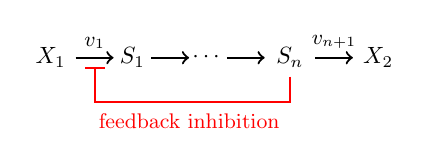
\begin{tikzpicture}[scale=0.8, every node/.style={scale=0.85}]
\node at (0,0) {$X_1$};
\draw[->, thick] (0.4,0) -- (1.0,0) node[midway, above] {\small $v_1$};
\node at (1.3,0) {$S_1$};
\draw[->, thick] (1.6,0) -- (2.2,0);
\node at (2.5,0) {$\cdots$};
\draw[->, thick] (2.8,0) -- (3.4,0);
\node at (3.8,0) {$S_n$};
\draw[->, thick] (4.2,0) -- (4.8,0) node[midway, above] {\small $v_{n+1}$};
\node at (5.2,0) {$X_2$};
% Feedback arrow
\draw[-|, thick, red] (3.8,-0.3) -- (3.8,-0.7) -- (0.7,-0.7) -- (0.7,-0.15);
\node[red] at (2.2,-1.0) {\small feedback inhibition};
\end{tikzpicture}
\end{center}

\textbf{Assumptions:}
\begin{itemize}
\item All reactions irreversible: $\varepsilon_{ii} = 0$
\item $S_n$ inhibits $v_1$: $\varepsilon_{1,n} < 0$
\end{itemize}

\subsection{Flux Control Coefficients}

\importantbox{
Internal enzymes have \textbf{zero} flux control:
\begin{equation*}
C_j^J = 0 \quad \text{for } j = 2, \ldots, n
\end{equation*}
}

Only $E_1$ and $E_{n+1}$ share flux control:
\begin{equation*}
C_1^J = \frac{\varepsilon_{n+1,n}}{\varepsilon_{n+1,n} - \varepsilon_{1,n}}, \quad C_{n+1}^J = \frac{-\varepsilon_{1,n}}{\varepsilon_{n+1,n} - \varepsilon_{1,n}}
\end{equation*}

\subsection{Control Ratio}

\begin{equation*}
\frac{C_{n+1}^J}{C_1^J} = -\frac{\varepsilon_{1,n}}{\varepsilon_{n+1,n}}
\end{equation*}

\textbf{Without feedback} ($\varepsilon_{1,n} = 0$): $C_1^J = 1$, $C_{n+1}^J = 0$

\textbf{Strong feedback} ($|\varepsilon_{1,n}| \gg |\varepsilon_{n+1,n}|$): Control shifts to $E_{n+1}$

\subsection{Concentration Control}

\textbf{First enzyme:}
\begin{equation*}
C_{i,1}^S = \frac{C_1^J}{\varepsilon_{i+1,i}} > 0 \quad (i = 1, \ldots, n)
\end{equation*}

\textbf{Last enzyme:}
\[
C_{i,n+1}^S = \begin{cases}
\dfrac{C_{n+1}^J}{\varepsilon_{i+1,i}} > 0 & \text{for } i \neq n \\[10pt]
-\dfrac{1}{\varepsilon_{n+1,n} - \varepsilon_{1,n}} < 0 & \text{for } i = n
\end{cases}
\]

\textbf{Internal enzymes} ($j = 2, \ldots, n$):
\begin{equation*}
C_{i,i+1}^S = -\frac{1}{\varepsilon_{i+1,i}} < 0
\end{equation*}
(Only control their own substrate concentration)

\subsection{Homeostasis Effect}

\importantbox{
Strong feedback ($|\varepsilon_{1,n}| \gg 1$):
\begin{align*}
C_{i,1}^S &\ll 1 \quad \text{(weak input control)} \\
|C_{n,n+1}^S| &\ll 1 \quad \text{(robust $S_n$ concentration)}
\end{align*}
}

\vspace{4pt}
This is the mathematical basis for homeostatic regulation in metabolic pathways.

% =============================================================================
\section{Summary Table}
% =============================================================================

\begin{center}
\footnotesize
\begin{tabular}{@{}lll@{}}
\toprule
\textbf{Quantity} & \textbf{Linear} & \textbf{General} \\
\midrule
Flux $J$ & Explicit (Eq.~5.88) & Implicit \\[5pt]
$C_j^J$ & $\displaystyle\dfrac{(1/k_j)\prod q}{\sum(1/k)\prod q}$ & $\displaystyle\dfrac{\prod(-\varepsilon/\varepsilon)}{1+\sum\prod}$ \\[14pt]
$C_{ij}^S$ & Via $C_j^J$ & Via connectivity \\[5pt]
$\sum C_j^J$ & $= 1$ & $= 1$ \\[5pt]
Sign of $C_j^J$ & $\geq 0$ always & $\geq 0$ (typical) \\
\bottomrule
\end{tabular}
\end{center}

% =============================================================================
\section{Quick Reference}
% =============================================================================

\textbf{Key relationships:}
\begin{enumerate}
\item $v_j = J$ at steady state (all rates equal)
\item $C_i^J/C_{i+1}^J = -\varepsilon_{i+1,i}/\varepsilon_{ii}$
\item Irreversible step shields downstream control
\item Feedback shifts control to output enzyme
\end{enumerate}

\textbf{Crossover theorem:}
\begin{itemize}
\item Activate enzyme $\Rightarrow$ decrease upstream $S$
\item Activate enzyme $\Rightarrow$ increase downstream $S$
\end{itemize}

\vfill
\hrule
\vspace{3pt}
\footnotesize
\textit{Created by Herbert M. Sauro, Based on: Heinrich \& Schuster, ``The Regulation of Cellular Systems'' (1996), Chapter 5.4.3, \today}

\end{multicols}
\end{document}
